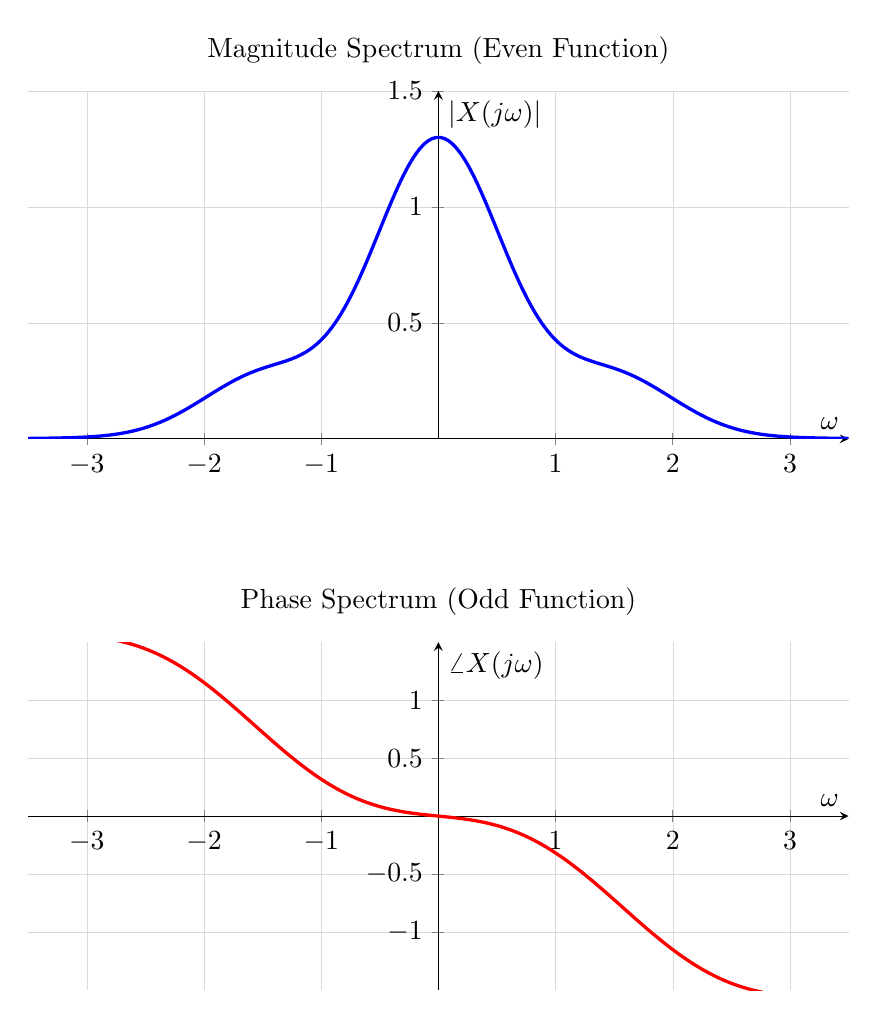
\begin{tikzpicture}
	% Define a common style for these plots
	\pgfplotsset{
		spec a/.style={
			width=12cm, height=6cm,
			axis lines=middle, xlabel={$\omega$},
			xmin=-3.5, xmax=3.5,
			xtick={-3, -2, -1, 1, 2, 3},
			grid=major, grid style={line width=.1pt, draw=gray!30},
			no marks,
		}
	}
	
	% Top plot: Magnitude
	\begin{scope}[yshift=7cm]
		\begin{axis}[
			spec a,
			title={Magnitude Spectrum (Even Function)},
			ylabel={$|X(j\omega)|$},
			ymin=0, ymax=1.5,
			ytick={0.5, 1, 1.5},
			]
			\addplot[blue, very thick, domain=-3.5:3.5, samples=200] {exp(-0.5*x^2) * (1 + 0.3*cos(deg(3*x)))};
		\end{axis}
	\end{scope}
	
	% Bottom plot: Phase
	\begin{scope}[yshift=0cm]
		\begin{axis}[
			spec a,
			title={Phase Spectrum (Odd Function)},
			ylabel={$\angle X(j\omega)$},
			ymin=-1.5, ymax=1.5,
			ytick={-1, -0.5, 0.5, 1},
			]
			\addplot[red, very thick, domain=-3.5:3.5, samples=200] {-0.5*x + 0.2*sin(deg(2*x))};
		\end{axis}
	\end{scope}
\end{tikzpicture}








